
%(BEGIN_QUESTION)
% Copyright 2006, Tony R. Kuphaldt, released under the Creative Commons Attribution License (v 1.0)
% This means you may do almost anything with this work of mine, so long as you give me proper credit

This P\&ID shows how two pressure transmitters may be linked with a radar level transmitter to provide data necessary to calculate not only liquid level, but also liquid density and total liquid mass stored in the vessel:

$$\includegraphics[width=15.5cm]{i00295x01.eps}$$

This is sometimes referred to as a {\it hybrid} level measurement system.  Explain what the word ``hybrid'' means in this context, and how these three transmitters accomplish the measurement objectives of liquid level, density, and total mass.  Also, explain what all the symbols mean in the P\&ID.

\vskip 10pt

\underbar{file i00295}
%(END_QUESTION)





%(BEGIN_ANSWER)

The use of two pressure transmitters, one at the bottom and one at the top, is reminiscent of a {\it hydrostatic tank expert} system (using three pressure sensors).  If this vessel were vented, we could get away with only using one pressure transmitter along with the radar gauge to calculate liquid level, density, and total mass.

%(END_ANSWER)





%(BEGIN_NOTES)

A fringe benefit of combining two completely different technologies for level measurement (radar + hydrostatic) is redundancy.  If one of these sensors fails, the other can still output data useful for determining the process level.  The level computer (UY-14) may be programmed to ``vote'' between one sensor or the other in the event of disparate measurements.

%INDEX% Measurement, level: radar + hydrostatic

%(END_NOTES)


